\begin{questions}
	\question{
		Presso il parcheggio del servizio di continuità assistenziale (guardia medica) di Perugia sono disponibili 4 postazioni auto: 
		\begin{itemize}
			\item una riservata al centralino (C)
			\item una riservata all'infermiere (I) di turno
			\item una riservata alla guardia medica (G) in servizio
			\item una riservata all'ambulanza (A) disponibile per questa sede
		\end{itemize}
		
		Nello stesso parcheggio sono presenti due pompe di rifornimento carburante che possono essere utilizzate secondo il seguente ordine di priorità: A $>$ G $>$ I $>$ C.\\
		
		Si chiede di progettare un sistema automatico per gestire la priorità di utilizzo delle pompe di rifornimento considerando che tutte le utilitarie potrebbero richiedere di fare rifornimento in contemporanea. 
	}

    \begin{solution}		
		\mysection{Specifica del comportamento}
		
		Il sistema di rifornimento è gestito tramite 4 differenti variabili ``L'', ``M'', ``N'' e ``O'', secondo la codifica riportata nella seguente tabella:
		
		\begin{table}[H]
			\centering
			\begin{tabular}{ |p{1cm}|p{1cm} |p{1cm}|p{1cm}| p{3cm}|  }
				\hline
				\multicolumn{5}{|c|}{Codifica utilizzo pompa di rifornimento} \\
				\hline
				L & M & N & O & Utilizzo\\
				\hline
				0 & 0 & 0 & 0 & Nessun utilizzo\\
				1 & 0 & 0 & 0 & A\\
				0 & 1 & 0 & 0 & G\\
				0 & 0 & 1 & 0 & I\\
				0 & 0 & 0 & 1 & C\\
				1 & 1 & 0 & 0 & AG\\
				1 & 0 & 1 & 0 & AI\\
				1 & 0 & 0 & 1 & AC\\
				0 & 1 & 1 & 0 & GI\\
				0 & 1 & 0 & 1 & GC\\
				0 & 0 & 1 & 1 & IC\\
				\hline
			\end{tabular}
			
			\label{tab:codifica}
		\end{table}
		
		\vspace{10em}

		\newpage
    
		\mysection{Formulazione}
		
		Creazione della tavola di verità per mostrare le relazioni tra input e output.
        
        \begin{center}
			\begin{tabular}{cccc|cccc|c}
				A & G & I & C 	& O & N & M & L & Utilizzo\\
				\hline
				0 & 0 & 0 & 0 	& 0 & 0 & 0 & 0 & Nessuno\\
				0 & 0 & 0 & 1 	& 1 & 0 & 0 & 0 & C\\
				0 & 0 & 1 & 0 	& 0 & 1 & 0 & 0 & I\\
				0 & 0 & 1 & 1 	& 1 & 1 & 0 & 0 & IC\\
				0 & 1 & 0 & 0 	& 0 & 0 & 1 & 0 & G\\ 
				0 & 1 & 0 & 1 	& 1 & 0 & 1 & 0 & GC\\
				0 & 1 & 1 & 0 	& 0 & 1 & 1 & 0 & GI\\
				0 & 1 & 1 & 1 	& 0 & 1 & 1 & 0 & GI\\
				1 & 0 & 0 & 0 	& 0 & 0 & 0 & 1 & A\\
				1 & 0 & 0 & 1 	& 1 & 0 & 0 & 1 & AC\\
				1 & 0 & 1 & 0 	& 0 & 1 & 0 & 1 & AI\\
				1 & 0 & 1 & 1 	& 0 & 1 & 0 & 1 & AI\\
				1 & 1 & 0 & 0 	& 0 & 0 & 1 & 1 & AG\\
				1 & 1 & 0 & 1 	& 0 & 0 & 1 & 1 & AG\\
				1 & 1 & 1 & 0 	& 0 & 0 & 1 & 1 & AG\\
				1 & 1 & 1 & 1 	& 0 & 0 & 1 & 1 & AG\\
			\end{tabular}
        \end{center}
        
        \newpage
            
        \mysection{Ottimizzazione}
        
        Creazione delle Mappe di Karnaugh per la semplificazione delle espressioni booleane.
            
            \begin{enumerate}
                \item Mappa di Karnaugh per ``O''.
                
                    \begin{center}
                        \begin{karnaugh-map}[4][4][1][$IC$][$AG$]
                            \manualterms{
                               	0,1,0,1,
                               	0,1,0,0,
                               	0,1,0,0,
                               	0,0,0,0}
                            \implicant{1}{5}
                            \implicant{1}{3}
                            \implicantedge{1}{1}{9}{9}
                         \end{karnaugh-map}
                    \end{center}
                    \[ O = \overline{AI}C +  \overline{GI}C + \overline{AG}C \]
                
				\vspace{1.5em}
				
                \item Mappa di Karnaugh per ``N''.
                
                    \begin{center}
                        \begin{karnaugh-map}[4][4][1][$IC$][$AG$]
                            \manualterms{                  0,0,1,1,
                               	0,0,1,1,
                               	0,0,1,1,
                               	0,0,0,0}
                            \implicant{3}{6}
                            \implicantedge{3}{2}{11}{10}
                         \end{karnaugh-map}
                    \end{center}
                \[ N = \overline{A}I + \overline{G}I \]
         
				\newpage
				
                \item Mappa di Karnaugh per ``M''.
                
                    \begin{center}
                        \begin{karnaugh-map}[4][4][1][$IC$][$AG$]
                            \manualterms{                  0,0,0,0,
                               	1,1,1,1,
                               	0,0,0,0,
                               	1,1,1,1}
                            \implicant{4}{14}
                         \end{karnaugh-map}
                    \end{center}
                \[ M = G \]
                
				\vspace{1.5em}
          						
                \item Mappa di Karnaugh per ``L''.
                
                 \begin{center}
                    	\begin{karnaugh-map}[4][4][1][$IC$][$AG$ ]
                    		\manualterms{                  0,0,0,0,
                    			0,0,0,0,
                    			1,1,1,1,
                    			1,1,1,1}
                    		\implicant{12}{10}
                    	\end{karnaugh-map}
                 \end{center}
                 \[ L = A \]                     
            \end{enumerate}
            
            \newpage
            
            \mysection{Generazione e disegno del circuito}
            Disegno del circuito combinatorio ottenuto dalle seguenti formule:
            
            \begin{align*}
            	O &= \overline{AI}C +  \overline{GI}C + \overline{AG}C\\
            	N &= \overline{A}I + \overline{G}I\\
            	M &= G \\
            	L &= A
            \end{align*}
            
            \begin{center}               	
                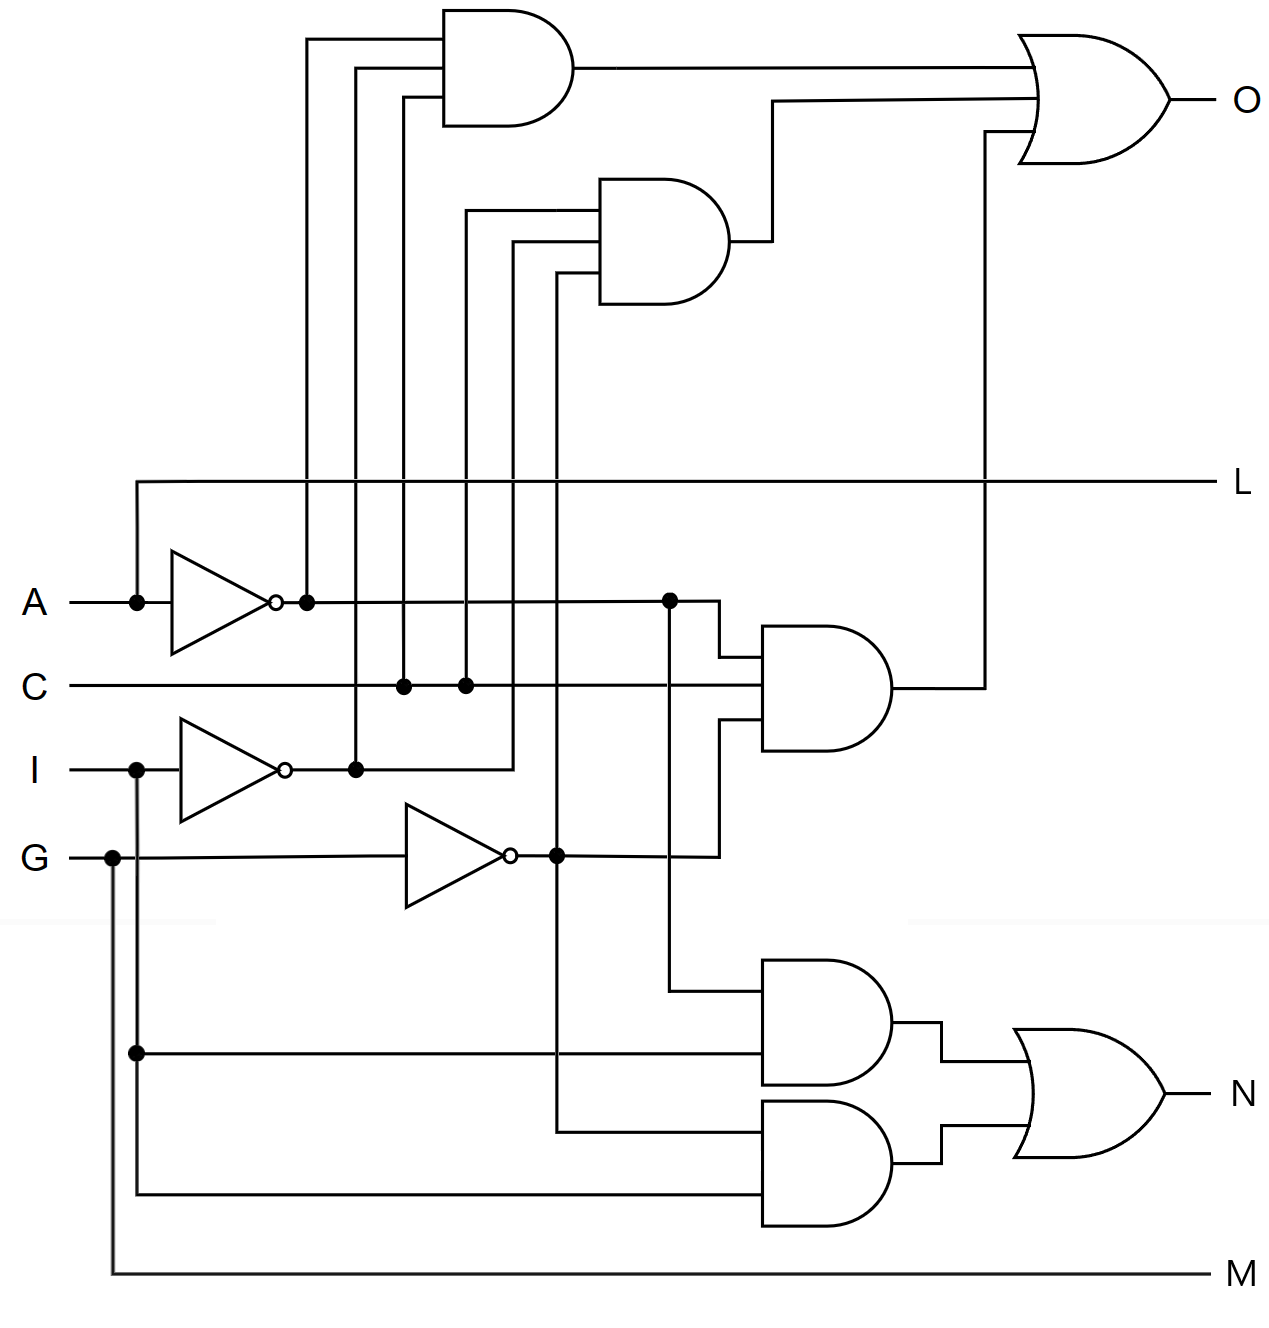
\includegraphics[width=13cm, keepaspectratio]{img/circuito_finale.png}
            \end{center}
            
            \newpage
            
            \mysection{Ottimizzazione del circuito}
            Per ottimizzare il circuito dobbiamo andare a trovare delle equazioni booleane equivalenti che costino meno di quelle che abbiamo attualmente.\\
            
            \vspace{-0.5em}
                        
            Per la variabile dipendente ``O'':\\
            \vspace{-1em}
            \begin{align}
            	O & = \overline{AI}C +  \overline{GI}C + \overline{AG}C \\            	
            	& = C(\overline{AI} +  \overline{GI} + \overline{AG})  &←~Raccolta~la~C\\            	
            	& = C((\overline{A} + \overline{I}) +(\overline{G} + \overline{I}) + (\overline{A} + \overline{G})) &←~Applicato~Demorgan\\            	
            	& = C(\overline{A} + \overline{G} + \overline{I}) &←~Applicato~teorema~Idempotenza
            \end{align}
            
            Possiamo notare come:
            \begin{itemize}
            	\item Per la funzione iniziale ($O = \overline{AI}C +  \overline{GI}C + \overline{AG}C$) si hanno i seguenti costi:
            	\begin{itemize}
            		\item Costo letterale = 9
            		\item Costo ingressi = 12
            	\end{itemize}
            	
            	\item Per la funzione minimizzata ($O = C(\overline{A} + \overline{G} + \overline{I})$) si ha la riduzione dei costi ai seguenti valori:
				\begin{itemize}
					\item Costo letterale = 4
					\item Costo ingressi = 5
				\end{itemize}
			\end{itemize}

            Per la variabile dipendente ``N'':\\
            \vspace{-1em}
			\begin{align}
				N &= \overline{A}I + \overline{G}I\\
				& = I(\overline{A} + \overline{G}) &←~Raccolta~la~I            	
			\end{align}   
			
            Possiamo notare come:
			\begin{itemize}
				\item Per la funzione iniziale ($N = \overline{A}I + \overline{G}I$) si hanno i seguenti costi:
				\begin{itemize}
					\item Costo letterale = 4
					\item Costo ingressi = 6
				\end{itemize}
				
				\item Per la funzione minimizzata ($N= I(\overline{A} + \overline{G})$) si ha la riduzione dei costi ai seguenti valori:
				\begin{itemize}
					\item Costo letterale = 3
					\item Costo ingressi = 4
				\end{itemize}
			\end{itemize}         
            
            
            \mysection{Generazione e disegno del circuito minimizzato}
            Disegniamo ora il circuito combinatorio minimizzato tramite le seguenti formule:
            \begin{align*}
                O &= C(\overline{A} + \overline{G} + \overline{I})\\
				N &= I(\overline{A} + \overline{G})\\
				M &= G \\
				L &= A
            \end{align*}   
            
            \vspace{-2em}
            
            \begin{center}
            	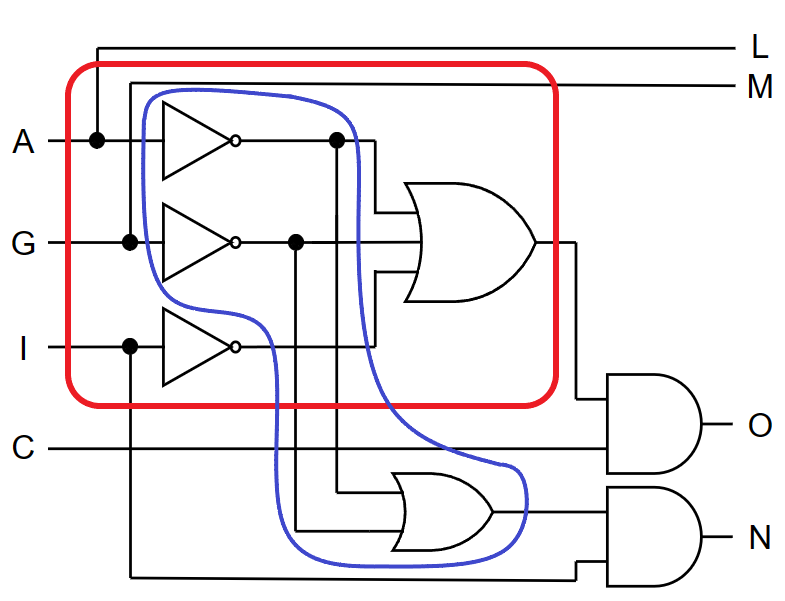
\includegraphics[width=9cm, keepaspectratio]{img/circuito_semi_minimizzato_2.png}
            \end{center}
            
            Notiamo però come sia possibile sostituire l'insieme di porte cerchiate in rosso e blu con due porte NAND in quanto aventi il medesimo comportamento. Possiamo quindi minimizzare ulteriormente la seguente funzione ottenendo il sottostante circuito:
            
            \vspace{-1.5em}
                        
            \begin{align*}
            	O &= C(\overline{A} + \overline{G} + \overline{I}) &=~& C(\overline{AGI}) 
            	&←~Applicato~Demorgan\\
            	N &= I(\overline{A} + \overline{G}) &=~& I(\overline{AG}) 
            	&←~Applicato~Demorgan
            \end{align*}    
            
            \vspace{-1.5em}

            \begin{center}
                    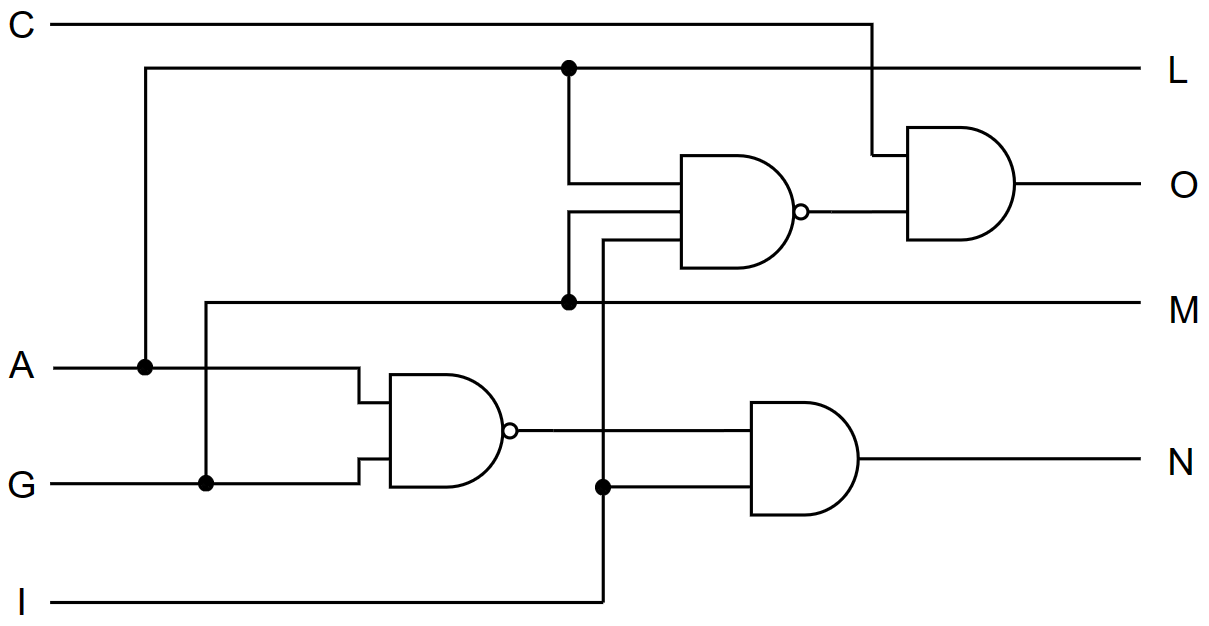
\includegraphics[width=13cm, keepaspectratio]{img/circuito_finale_minimizzato.png}
            \end{center}
    \end{solution}
\end{questions}